% Autoría principal: Mera; respaldar con archivos REALES.
\subsection{Implementación con gRPC y Protocol Buffers}

En la versión gRPC, cada nodo publica un servicio remoto y el cliente invoca un método de ese servicio como si fuera una función local. El intercambio es el mismo que en TCP: el emisor envía \texttt{sender}, \texttt{timestamp} y \texttt{message}, y el receptor responde con \texttt{receiver}, \texttt{timestamp} y \texttt{ok}. La diferencia está en quién construye y lee los mensajes. En TCP el programa arma el JSON, lo delimita con un salto de línea y valida cada campo; en gRPC esa tarea la hacen las clases generadas a partir del contrato \texttt{.proto}, que serializan los datos en formato binario y los envían sobre HTTP/2 \cite{niswar2024grpc,sliwa2021grpc}.

El código está en \texttt{src/grpc/}:
\begin{itemize}
	\item \texttt{messaging.proto}: contrato del servicio y de los mensajes.
	\item \texttt{messaging\_pb2.py} y \texttt{messaging\_pb2\_grpc.py}: código generado con \texttt{grpcio-tools}; no se edita a mano.
	\item \texttt{server\_grpc.py}: servidor de un nodo (\texttt{nodo-A}, \texttt{nodo-B} o \texttt{nodo-C}, en los puertos 5000, 5001 y 5002).
	\item \texttt{client\_grpc.py}: cliente con la misma interfaz que el cliente TCP (\texttt{conectar}, \texttt{enviar}, \texttt{cerrar}).
	\item \texttt{registro\_grpc.py}: escritura de eventos y latencias en CSV, con las mismas columnas que el registro TCP.
\end{itemize}
El reloj lógico no se implementó por separado: tanto el servidor como el cliente usan la clase \texttt{LamportClock} de \texttt{src/common/lamport.py}, la misma que usa TCP y que se describe en la implementación del reloj de Lamport.

\subsubsection{Contrato de servicio (.proto)}

El contrato define un servicio con un único procedimiento remoto, \texttt{EnviarMensaje}, que recibe un \texttt{Request} y devuelve un \texttt{Response}. Los nombres del servicio y de los mensajes siguen la guía de la práctica, y los campos son los mismos que se acordaron para el JSON de TCP.

\begin{lstlisting}[caption={Contrato \texttt{src/grpc/messaging.proto}}]
	syntax = "proto3";
	
	package messaging;
	
	service MessagingService {
		rpc EnviarMensaje (Request) returns (Response);
	}
	
	message Request {
		string sender = 1;
		int64 timestamp = 2;
		string message = 3;
	}
	
	message Response {
		string receiver = 1;
		int64 timestamp = 2;
		bool ok = 3;
	}
\end{lstlisting}

Los números \texttt{= 1}, \texttt{= 2} y \texttt{= 3} no son valores, sino las etiquetas con las que cada campo viaja en el mensaje binario; por eso el nombre del campo no se transmite y las etiquetas no deben cambiarse una vez publicado el contrato. El reloj se declaró como \texttt{int64} porque es un contador entero que solo crece. El código Python se generó desde \texttt{src/grpc/} con el comando indicado en la guía:

\begin{lstlisting}[language=bash,caption={Generación del código a partir del contrato}]
	python -m grpc_tools.protoc -I. --python_out=. --grpc_python_out=. messaging.proto
\end{lstlisting}

Para ver el efecto de la codificación binaria, se serializó el mismo contenido con Protocol Buffers y con el JSON compacto que usa el cliente TCP. La tabla~\ref{tab:tamanos-serializados} muestra el tamaño de cada mensaje sin contar el salto de línea que TCP añade como delimitador ni las cabeceras de HTTP/2. La diferencia es de 33 o 34 bytes por solicitud: pesa en mensajes cortos, pero en uno de 10\,KB representa menos del 0,4\,\%.

\par\medskip
\noindent\begin{minipage}{\linewidth}
	\centering
	\makeatletter\def\@captype{table}\makeatother
	\caption{Tamaño serializado de una solicitud y un acuse (bytes)}
	\label{tab:tamanos-serializados}
	\begin{tabular}{@{}lrr@{}}
		\toprule
		Contenido & Protocol Buffers & JSON compacto \\
		\midrule
		Solicitud con \texttt{message = "hola"} & 16 & 50 \\
		Solicitud con carga de 100 bytes & 112 & 146 \\
		Solicitud con carga de 10\,240 bytes & 10\,253 & 10\,286 \\
		Acuse (\texttt{receiver}, \texttt{timestamp = 79}, \texttt{ok}) & 12 & 46 \\
		\bottomrule
	\end{tabular}
\end{minipage}
\par\medskip

\subsubsection{Servidor}

El servidor crea un \texttt{grpc.server} con un grupo de diez hilos, registra el servicio y escucha en \texttt{127.0.0.1} en el puerto de su nodo. Se usa la dirección IPv4 en lugar de \texttt{localhost} para que Windows no intente primero IPv6, lo que añadiría retrasos a las mediciones. Cuando llega una solicitud, el método \texttt{EnviarMensaje} aplica dos eventos de Lamport: la recepción y el envío del acuse.

\begin{lstlisting}[language=Python,caption={Atención de una solicitud en \texttt{server\_grpc.py}}]
	def EnviarMensaje(self, request, context):
	try:
	ts_recepcion = self.reloj.receive(request.timestamp)
	except (TypeError, ValueError) as error:
	context.abort(grpc.StatusCode.INVALID_ARGUMENT, str(error))
	id_mensaje = self._siguiente_id(context.peer(), request.sender)
	# ... registro de recepcion_solicitud ...
	ts_acuse = self.reloj.tick()
	# ... registro de envio_acuse ...
	return messaging_pb2.Response(receiver=self.nombre, timestamp=ts_acuse, ok=True)
\end{lstlisting}

Al recibir se aplica $\max(\text{local}, \text{recibido}) + 1$. Responder con el acuse es un evento nuevo, por lo que se incrementa el reloj una vez más y ese valor es el que viaja en el \texttt{Response}; así se comporta también el servidor TCP. El identificador del mensaje se calcula por conexión (\texttt{context.peer()}) y por emisor, con el formato \texttt{nodo-A-000001}, para que coincida con el que genera el cliente y se pueda emparejar cada envío con su recepción en la verificación de Lamport. La opción \texttt{--silencioso} desactiva la impresión en consola y el registro de eventos, de modo que en las mediciones no se cuente el tiempo de escribir en pantalla o en disco.

\subsubsection{Cliente y medición de la latencia}

El cliente abre un solo canal en \texttt{conectar} y lo reutiliza para todos los envíos de la corrida. Antes de devolver el control espera a que el canal esté listo (\texttt{grpc.channel\_ready\_future}), para que el establecimiento de la conexión no quede dentro de la latencia del primer mensaje. El método \texttt{enviar} recibe los mismos parámetros que el de \texttt{ClienteTCP}, lo que permite que \texttt{analysis/benchmark.py} use cualquiera de los dos clientes sin cambiar el procedimiento de medición.

\begin{lstlisting}[language=Python,caption={Envío y medición del RTT en \texttt{client\_grpc.py}}]
	ts_envio = self.clock.send()
	# ... registro de envio_solicitud (fuera del tiempo medido) ...
	solicitud = messaging_pb2.Request(sender=sender, timestamp=ts_envio, message=message)
	inicio = time.perf_counter()
	acuse = self.stub.EnviarMensaje(solicitud, timeout=self.timeout)
	latencia_ms = (time.perf_counter() - inicio) * 1000
	ts_recepcion = self.clock.receive(acuse.timestamp)
\end{lstlisting}

El tiempo medido comprende la serialización de la solicitud, el viaje de ida y vuelta, la atención en el servidor y la deserialización del acuse. La escritura en CSV se hace antes y después de ese intervalo. La carga útil se genera con la misma función que en TCP (\texttt{"x" * tamano}), de modo que los mensajes de 100 y 10\,240 bytes son idénticos en ambos mecanismos.

\subsubsection{Manejo de errores}

En TCP los errores llegan como excepciones del socket y los campos del JSON se validan a mano. En gRPC, el contrato ya garantiza los tipos: un \texttt{timestamp} siempre llega como entero. Lo que sí debe validarse es el valor, y los fallos de comunicación se reportan con códigos de estado de gRPC. La tabla~\ref{tab:errores-grpc} resume cómo se tratan.

\par\medskip
\noindent\begin{minipage}{\linewidth}
	\centering
	\makeatletter\def\@captype{table}\makeatother
	\caption{Tratamiento de errores en la implementación gRPC}
	\label{tab:errores-grpc}
	\begin{tabularx}{\linewidth}{@{}>{\raggedright\arraybackslash}X >{\raggedright\arraybackslash}p{3.6cm} >{\raggedright\arraybackslash}p{3.2cm}@{}}
		\toprule
		Situación & Respuesta del código & Registro en CSV \\
		\midrule
		El \texttt{timestamp} recibido es negativo & \texttt{INVALID\_ARGUMENT} desde el servidor, que sigue en marcha & --- \\
		El nodo destino está apagado al conectar & El cliente informa que no pudo conectar tras 2\,s & --- \\
		La llamada supera el límite de 2\,s & \texttt{DEADLINE\_EXCEEDED} & \texttt{ok = false}, \texttt{timeout} \\
		El servidor deja de estar disponible & \texttt{UNAVAILABLE} & \texttt{ok = false}, \texttt{conexion\_rechazada} \\
		Cualquier otro código & El error se informa y se continúa con el siguiente envío & \texttt{ok = false}, \texttt{otro} \\
		\bottomrule
	\end{tabularx}
\end{minipage}
\par\medskip

Los dos primeros casos se comprobaron el 19 de noviembre de 2026: un envío con \texttt{timestamp = -1} devolvió \texttt{INVALID\_ARGUMENT} con el mensaje «El timestamp no puede ser negativo», y un envío a \texttt{nodo-C} apagado terminó con «No se pudo conectar con nodo-C en 127.0.0.1:5002», mientras \texttt{nodo-B} seguía respondiendo (figura~\ref{fig:grpc-nodo-caido}). Los otros tres casos están contemplados en el código, pero no se provocaron durante las pruebas. Los nombres \texttt{timeout}, \texttt{conexion\_rechazada} y \texttt{otro} son los mismos que se acordaron para TCP, de modo que el análisis puede agrupar los errores de ambos mecanismos.

\par\medskip
\noindent\begin{minipage}{\linewidth}
	\centering
	\makeatletter\def\@captype{figure}\makeatother
	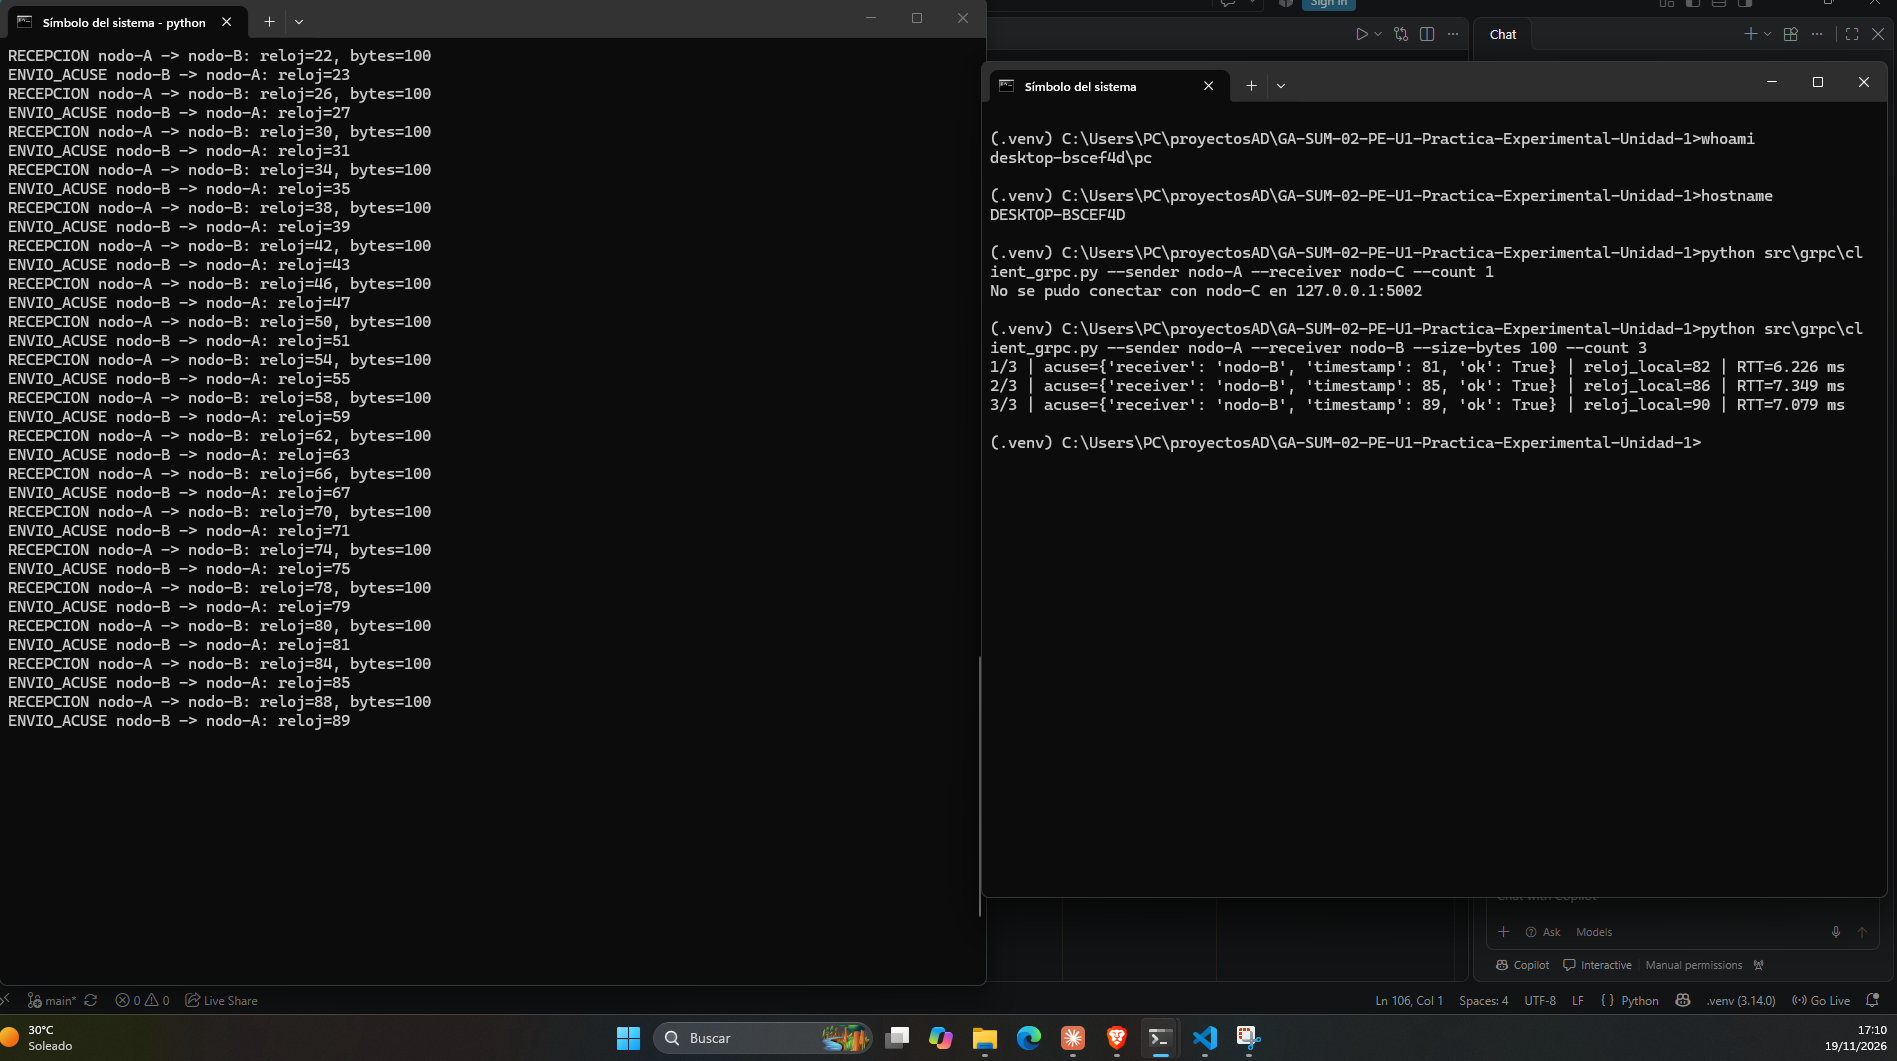
\includegraphics[width=\linewidth]{evidencias/Mera/grpc_nodo_caido_2026-11-19.png}
	\caption{Envío a \texttt{nodo-C} apagado y envíos correctos a \texttt{nodo-B} en la misma sesión.}
	\label{fig:grpc-nodo-caido}
\end{minipage}
\par\medskip

\subsubsection{Ejecución de 20 intercambios y registro de eventos}

Los 20 intercambios se ejecutaron el 19 de noviembre de 2026 con las mismas condiciones que la prueba TCP: servidor en \texttt{nodo-B}, cliente en \texttt{nodo-A}, carga de 100 bytes y corrida 0 (prueba funcional).

\begin{lstlisting}[language=bash,caption={Comandos de la prueba de 20 intercambios}]
	python src\grpc\server_grpc.py nodo-B
	python src\grpc\client_grpc.py --sender nodo-A --receiver nodo-B --size-bytes 100 --count 20 --run 0
\end{lstlisting}

Los 20 envíos recibieron acuse con \texttt{ok = True} (figura~\ref{fig:grpc-20}). En el primer intercambio, \texttt{nodo-A} envió con reloj 1, \texttt{nodo-B} registró la recepción con 2 y el envío del acuse con 3, y \texttt{nodo-A} quedó en 4 al recibirlo. Cada intercambio suma cuatro eventos, por lo que el último acuse llevó el valor 79 y el reloj de \texttt{nodo-A} terminó en 80. Es la misma secuencia que se obtuvo con TCP, lo que confirma que ambos mecanismos aplican las reglas de Lamport en el mismo orden; el transporte no cambia el resultado del reloj lógico. Las latencias de esta corrida (entre 6 y 32\,ms) no se usan en los resultados, porque el servidor imprimía y escribía en CSV en cada solicitud; las mediciones oficiales se obtuvieron con \texttt{analysis/benchmark.py} (sección de protocolo experimental).

\par\medskip
\noindent\begin{minipage}{\linewidth}
	\centering
	\makeatletter\def\@captype{figure}\makeatother
	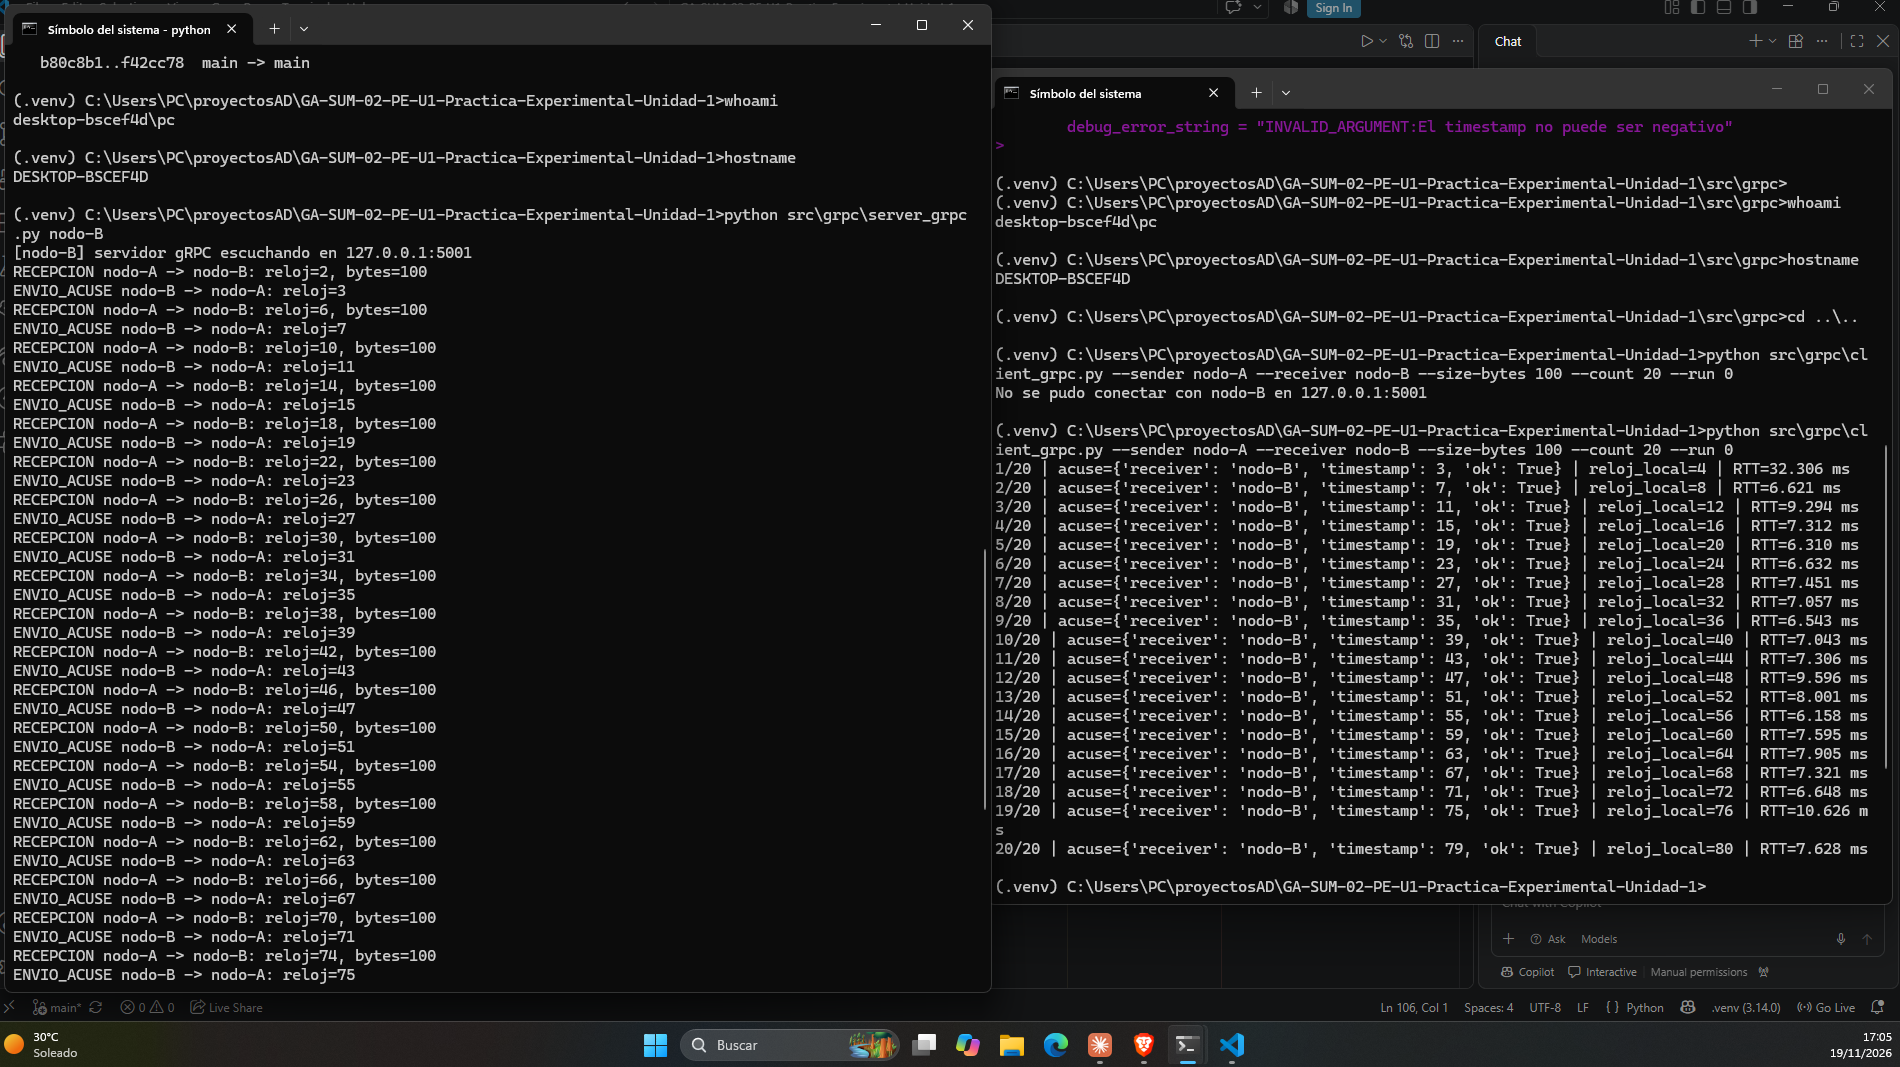
\includegraphics[width=\linewidth]{evidencias/Mera/grpc_20_intercambios_2026-11-19.png}
	\caption{Servidor gRPC de \texttt{nodo-B} (izquierda) y cliente de \texttt{nodo-A} (derecha) durante los 20 intercambios.}
	\label{fig:grpc-20}
\end{minipage}
\par\medskip

\pendiente{Indicar el archivo CSV de eventos gRPC de la corrida oficial que se usa en la verificación de Lamport, cuando el equipo lo genere y lo registre en SHA256SUMS. Los CSV de la corrida funcional del 19 de noviembre no se conservaron.}